% Options for packages loaded elsewhere
\PassOptionsToPackage{unicode}{hyperref}
\PassOptionsToPackage{hyphens}{url}
\PassOptionsToPackage{dvipsnames,svgnames,x11names}{xcolor}
%
\documentclass[
  11pt,
  a4paper,
  DIV=11,
  numbers=noendperiod]{scrartcl}

\usepackage{amsmath,amssymb}
\usepackage{iftex}
\ifPDFTeX
  \usepackage[T1]{fontenc}
  \usepackage[utf8]{inputenc}
  \usepackage{textcomp} % provide euro and other symbols
\else % if luatex or xetex
  \usepackage{unicode-math}
  \defaultfontfeatures{Scale=MatchLowercase}
  \defaultfontfeatures[\rmfamily]{Ligatures=TeX,Scale=1}
\fi
\usepackage{lmodern}
\ifPDFTeX\else  
    % xetex/luatex font selection
\fi
% Use upquote if available, for straight quotes in verbatim environments
\IfFileExists{upquote.sty}{\usepackage{upquote}}{}
\IfFileExists{microtype.sty}{% use microtype if available
  \usepackage[]{microtype}
  \UseMicrotypeSet[protrusion]{basicmath} % disable protrusion for tt fonts
}{}
\makeatletter
\@ifundefined{KOMAClassName}{% if non-KOMA class
  \IfFileExists{parskip.sty}{%
    \usepackage{parskip}
  }{% else
    \setlength{\parindent}{0pt}
    \setlength{\parskip}{6pt plus 2pt minus 1pt}}
}{% if KOMA class
  \KOMAoptions{parskip=half}}
\makeatother
\usepackage{xcolor}
\usepackage[margin=1in]{geometry}
\setlength{\emergencystretch}{3em} % prevent overfull lines
\setcounter{secnumdepth}{5}
% Make \paragraph and \subparagraph free-standing
\makeatletter
\ifx\paragraph\undefined\else
  \let\oldparagraph\paragraph
  \renewcommand{\paragraph}{
    \@ifstar
      \xxxParagraphStar
      \xxxParagraphNoStar
  }
  \newcommand{\xxxParagraphStar}[1]{\oldparagraph*{#1}\mbox{}}
  \newcommand{\xxxParagraphNoStar}[1]{\oldparagraph{#1}\mbox{}}
\fi
\ifx\subparagraph\undefined\else
  \let\oldsubparagraph\subparagraph
  \renewcommand{\subparagraph}{
    \@ifstar
      \xxxSubParagraphStar
      \xxxSubParagraphNoStar
  }
  \newcommand{\xxxSubParagraphStar}[1]{\oldsubparagraph*{#1}\mbox{}}
  \newcommand{\xxxSubParagraphNoStar}[1]{\oldsubparagraph{#1}\mbox{}}
\fi
\makeatother


\providecommand{\tightlist}{%
  \setlength{\itemsep}{0pt}\setlength{\parskip}{0pt}}\usepackage{longtable,booktabs,array}
\usepackage{calc} % for calculating minipage widths
% Correct order of tables after \paragraph or \subparagraph
\usepackage{etoolbox}
\makeatletter
\patchcmd\longtable{\par}{\if@noskipsec\mbox{}\fi\par}{}{}
\makeatother
% Allow footnotes in longtable head/foot
\IfFileExists{footnotehyper.sty}{\usepackage{footnotehyper}}{\usepackage{footnote}}
\makesavenoteenv{longtable}
\usepackage{graphicx}
\makeatletter
\def\maxwidth{\ifdim\Gin@nat@width>\linewidth\linewidth\else\Gin@nat@width\fi}
\def\maxheight{\ifdim\Gin@nat@height>\textheight\textheight\else\Gin@nat@height\fi}
\makeatother
% Scale images if necessary, so that they will not overflow the page
% margins by default, and it is still possible to overwrite the defaults
% using explicit options in \includegraphics[width, height, ...]{}
\setkeys{Gin}{width=\maxwidth,height=\maxheight,keepaspectratio}
% Set default figure placement to htbp
\makeatletter
\def\fps@figure{htbp}
\makeatother
% definitions for citeproc citations
\NewDocumentCommand\citeproctext{}{}
\NewDocumentCommand\citeproc{mm}{%
  \begingroup\def\citeproctext{#2}\cite{#1}\endgroup}
\makeatletter
 % allow citations to break across lines
 \let\@cite@ofmt\@firstofone
 % avoid brackets around text for \cite:
 \def\@biblabel#1{}
 \def\@cite#1#2{{#1\if@tempswa , #2\fi}}
\makeatother
\newlength{\cslhangindent}
\setlength{\cslhangindent}{1.5em}
\newlength{\csllabelwidth}
\setlength{\csllabelwidth}{3em}
\newenvironment{CSLReferences}[2] % #1 hanging-indent, #2 entry-spacing
 {\begin{list}{}{%
  \setlength{\itemindent}{0pt}
  \setlength{\leftmargin}{0pt}
  \setlength{\parsep}{0pt}
  % turn on hanging indent if param 1 is 1
  \ifodd #1
   \setlength{\leftmargin}{\cslhangindent}
   \setlength{\itemindent}{-1\cslhangindent}
  \fi
  % set entry spacing
  \setlength{\itemsep}{#2\baselineskip}}}
 {\end{list}}
\usepackage{calc}
\newcommand{\CSLBlock}[1]{\hfill\break\parbox[t]{\linewidth}{\strut\ignorespaces#1\strut}}
\newcommand{\CSLLeftMargin}[1]{\parbox[t]{\csllabelwidth}{\strut#1\strut}}
\newcommand{\CSLRightInline}[1]{\parbox[t]{\linewidth - \csllabelwidth}{\strut#1\strut}}
\newcommand{\CSLIndent}[1]{\hspace{\cslhangindent}#1}

\KOMAoption{captions}{tableheading,figureheading}
\makeatletter
\@ifpackageloaded{caption}{}{\usepackage{caption}}
\AtBeginDocument{%
\ifdefined\contentsname
  \renewcommand*\contentsname{Table of contents}
\else
  \newcommand\contentsname{Table of contents}
\fi
\ifdefined\listfigurename
  \renewcommand*\listfigurename{List of Figures}
\else
  \newcommand\listfigurename{List of Figures}
\fi
\ifdefined\listtablename
  \renewcommand*\listtablename{List of Tables}
\else
  \newcommand\listtablename{List of Tables}
\fi
\ifdefined\figurename
  \renewcommand*\figurename{Figure}
\else
  \newcommand\figurename{Figure}
\fi
\ifdefined\tablename
  \renewcommand*\tablename{Table}
\else
  \newcommand\tablename{Table}
\fi
}
\@ifpackageloaded{float}{}{\usepackage{float}}
\floatstyle{ruled}
\@ifundefined{c@chapter}{\newfloat{codelisting}{h}{lop}}{\newfloat{codelisting}{h}{lop}[chapter]}
\floatname{codelisting}{Listing}
\newcommand*\listoflistings{\listof{codelisting}{List of Listings}}
\makeatother
\makeatletter
\makeatother
\makeatletter
\@ifpackageloaded{caption}{}{\usepackage{caption}}
\@ifpackageloaded{subcaption}{}{\usepackage{subcaption}}
\makeatother

\ifLuaTeX
  \usepackage{selnolig}  % disable illegal ligatures
\fi
\usepackage{bookmark}

\IfFileExists{xurl.sty}{\usepackage{xurl}}{} % add URL line breaks if available
\urlstyle{same} % disable monospaced font for URLs
\hypersetup{
  pdftitle={Menu Engineering Supercharged},
  pdfauthor={Hankun Xiao, Yasmin Hassan, Jessie Zhang, Zhiwei Zhang},
  colorlinks=true,
  linkcolor={blue},
  filecolor={Maroon},
  citecolor={Blue},
  urlcolor={Blue},
  pdfcreator={LaTeX via pandoc}}


\title{Menu Engineering Supercharged}
\usepackage{etoolbox}
\makeatletter
\providecommand{\subtitle}[1]{% add subtitle to \maketitle
  \apptocmd{\@title}{\par {\large #1 \par}}{}{}
}
\makeatother
\subtitle{MDS Capstone Final Report}
\author{Hankun Xiao, Yasmin Hassan, Jessie Zhang, Zhiwei Zhang}
\date{}

\begin{document}
\maketitle

\renewcommand*\contentsname{Table of contents}
{
\hypersetup{linkcolor=}
\setcounter{tocdepth}{2}
\tableofcontents
}

\section{Executive Summary}\label{executive-summary}

This project supports our partner, Heymate, in delivering data-driven
menu insights to their restaurant clients. Leveraging over 3 million
popularity records and the power of large language models, we developed
a structured data cleaning pipeline and generated a weighted scoring
mechanism to identify top-performing dishes. The final product includes
a scalable recommendation system that suggests the most popular menu
items based on restaurant type, enabling merchants to optimize their
offerings with minimal technical effort.

\section{Introduction}\label{introduction}

Our capstone partner, Heymate, offers an all-in-one business management
platform, primarily serving restaurant clients. However, many of these
restaurant owners struggle to design menus that align with customer
preferences and evolving market trends due to limited access to broader
market data. Our project aims to bridge that gap by transforming
publicly available menu data into structured insights that support
data-informed menu design, enabling the partner to deliver greater value
to its clients through market-driven recommendations.

Our initial resource was internal database provided by Heymate,
containing thousands of raw menu records from their clients. However,
the internal data alone was insufficient to support robust
recommendation modeling due to limited scale of menu and lack of
trending information. To address this, we explored various open-source
datasets, and found a menu dataset containing millions of menu records
along with associated popularity metrics on Uber Eats (Sakib (2023)),
making it a strong data source in terms of scale, quality, and coverage.

However, messy data, large-scale datasets, and customized menu item
names posed significant challenges to the construction of our
recommendation system. Therefore, our scientific objective was to design
an end-to-end pipeline that leverages diverse data science techniques to
build a robust and scalable recommendation system, powered by a
popularity-based knowledge base and capable of handling multi-type
inputs.

\newpage

\section{Data Pipeline Framework}\label{data-pipeline-framework}

Based on the project objective, we developed the following modular data
pipeline framework: (Figure~\ref{fig-data-pipeline-overview})

\begin{figure}

\caption{\label{fig-data-pipeline-overview}Data Pipeline Framework - The
core recommender supported by two pipelines: one for modeling from
market data, and another for generating recommendations}

\centering{

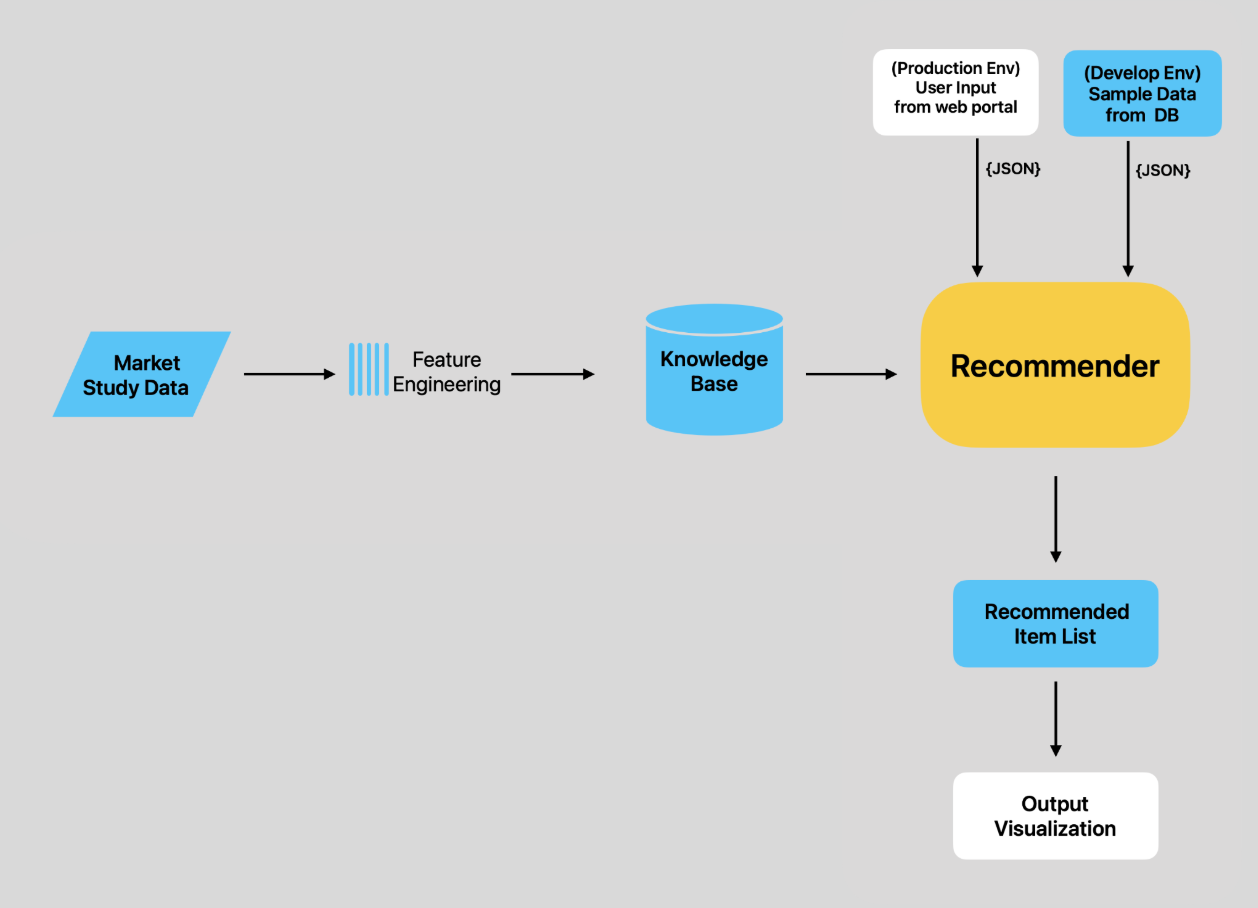
\includegraphics[width=0.8\textwidth,height=\textheight]{../image/final_1_data_pipeline_overview.png}

}

\end{figure}%

\subsection{Model Input Pipeline (Horizontal
Workflow)}\label{model-input-pipeline-horizontal-workflow}

\begin{enumerate}
\def\labelenumi{\arabic{enumi}.}
\tightlist
\item
  Data Ingestion: After researching across multiple open-source
  datasets, we found a Uber Eats dataset from Kaggle covers a wide range
  of restaurant types, menu items, and their corresponding descriptions.
\item
  Feature Engineering: As the raw dataset was quite messy, it needed to
  undergo a series of preprocessing and standardization process so that
  we can use them for further popularity score calculation.
\item
  Knowledge Base Construction: Under suggestion and domain knowledge
  from the project partner,we buily a weighted scoring knowledge base on
  various popularity metrics. This serves as the foundation for
  capturing market trends and powering recommendations.
\end{enumerate}

\subsection{Testing and Production Pipeline (Vertical
Workflow)}\label{testing-and-production-pipeline-vertical-workflow}

\begin{enumerate}
\def\labelenumi{\arabic{enumi}.}
\tightlist
\item
  Recommender Input: The recommender system can process JSON inputs from
  two sources, including client restaurant type from Heymate internal
  database, and user input of restaurant types via the web portal for
  real-time recommendations.
\item
  Recommendation Module: Based on the specified restaurant type, the
  engine searches the knowledge base, ranks menu items using scoring
  logic, and generates a tailored Recommended Item List.
\item
  Output Visualization: Final recommendations are displayed through a
  user-friendly dashboard, enabling clear interpretation and easy action
  on the results.
\end{enumerate}

\section{Transition from Framework to Data
Product}\label{transition-from-framework-to-data-product}

Having established our framework, we shifted our focus to building a
scalable data product. At its core is a recommendation engine that
suggests top-performing dishes by leveraging aggregated popularity
patterns from similar restaurant types.

\subsection{Data Wrangling Module}\label{data-wrangling-module}

\subsubsection{Exploratory Data
Analysis}\label{exploratory-data-analysis}

To support the development of a robust recommendation engine, we first
conducted exploratory data analysis (EDA) to assess data quality and
structure. The insights suggest the need to perform wrangling tasks for
a clean, consistent, and high-quality model input dataset.

\begin{enumerate}
\def\labelenumi{\arabic{enumi}.}
\tightlist
\item
  \textbf{Data Quality and Inconsistencies:} The raw Uber Eats data
  contains more than 5 million menu records, but it presented
  significant quality issues (shown in Table~\ref{tbl-null-entries}),
  including missing critical metrics, formatting inconsistencies, posing
  a major challenge in popularity score calculation. Therefore, we
  implemented preprocessing logic to remove all these incomplete,
  duplicated, or other invalid menu records, which results in around 3.2
  million records for next step.
\end{enumerate}

\begin{longtable}[]{@{}lr@{}}
\caption{Null Entries in Uber Eats dataset (Model Input
Data)}\label{tbl-null-entries}\tabularnewline
\toprule\noalign{}
column\_name & null\_count \\
\midrule\noalign{}
\endfirsthead
\toprule\noalign{}
column\_name & null\_count \\
\midrule\noalign{}
\endhead
\bottomrule\noalign{}
\endlastfoot
id & 0 \\
restaurant\_name & 0 \\
score & 1958476 \\
ratings & 1958476 \\
restaurant\_type & 2499 \\
full\_address & 33745 \\
menu\_category & 160 \\
menu\_name & 164 \\
menu\_item\_description & 1452305 \\
price & 160 \\
\end{longtable}

\begin{enumerate}
\def\labelenumi{\arabic{enumi}.}
\setcounter{enumi}{1}
\tightlist
\item
  \textbf{Large-Scale Data Processing:} Even after preprocessing, the
  dataset still contained over \textbf{3 million} records, making full
  in-memory processing impractical due to runtime and memory
  constraints. To ensure scalability, we implemented batch processing by
  retrieving indexed chunks and deployed it via a Flask framework with
  multithreaded API calls for concurrent execution.
\end{enumerate}

\newpage

\begin{enumerate}
\def\labelenumi{\arabic{enumi}.}
\setcounter{enumi}{2}
\tightlist
\item
  \textbf{Menu Naming Variability:} The biggest challenge was the
  inconsistent naming of similar dishes, for example, ``seafood fried
  rice'' appeared in various forms and languages
  (Figure~\ref{fig-seafood-fried-rice-var}). This hindered similarity
  comparisons and recommendation accuracy. To address this, we used
  OpenAI's GPT API for semantic standardization, enhancing consistency
  and model performance.
\end{enumerate}

\begin{figure}

\caption{\label{fig-seafood-fried-rice-var}Seafood Fried Rice Spelling
Variation}

\centering{

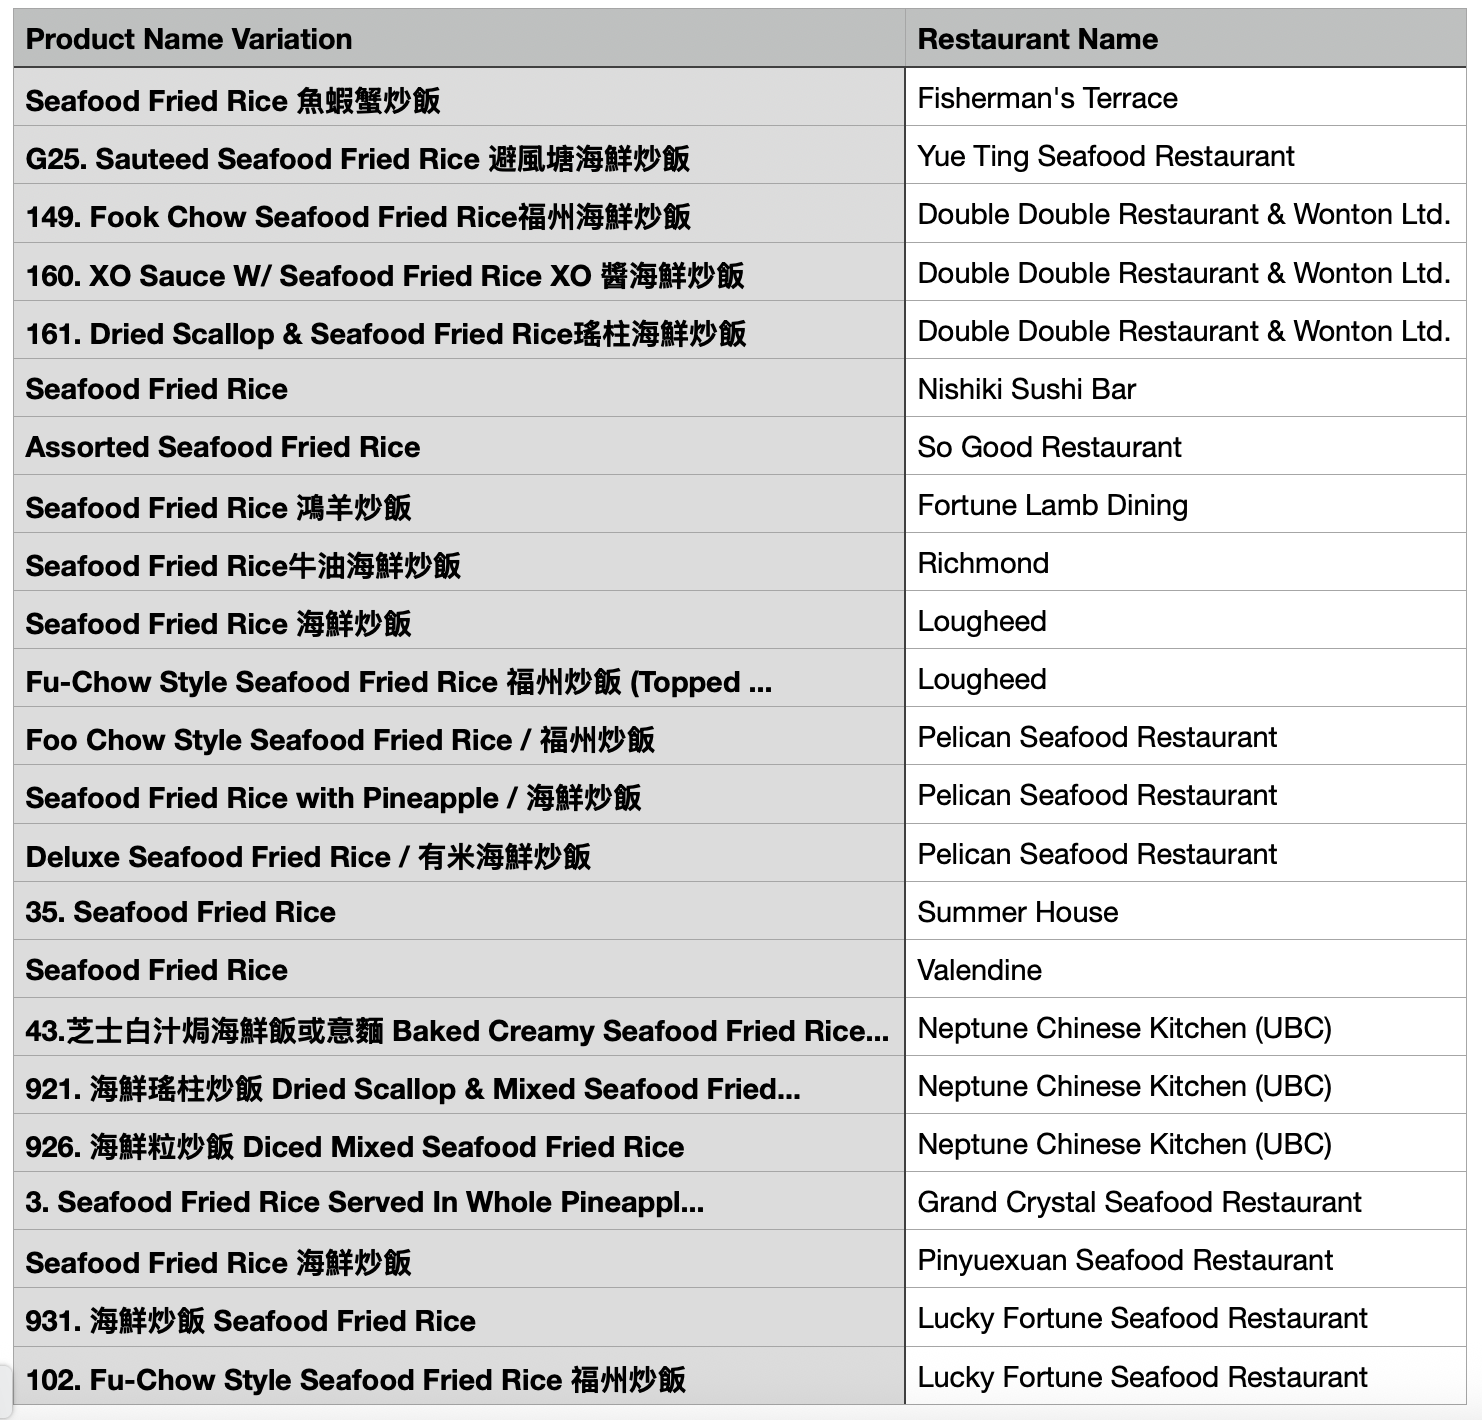
\includegraphics[width=0.8\textwidth,height=\textheight]{../image/final-6-seafood_fried_rice_products.png}

}

\end{figure}%

\subsubsection{Solution Pipeline}\label{solution-pipeline}

All wrangling tasks were encapsulated in modular Python scripts and
integrated into a unified data pipeline
(Figure~\ref{fig-training-pipline}). This pipeline includes:

\begin{figure}

\caption{\label{fig-training-pipline}Solution Pipeline (Model Training)}

\centering{

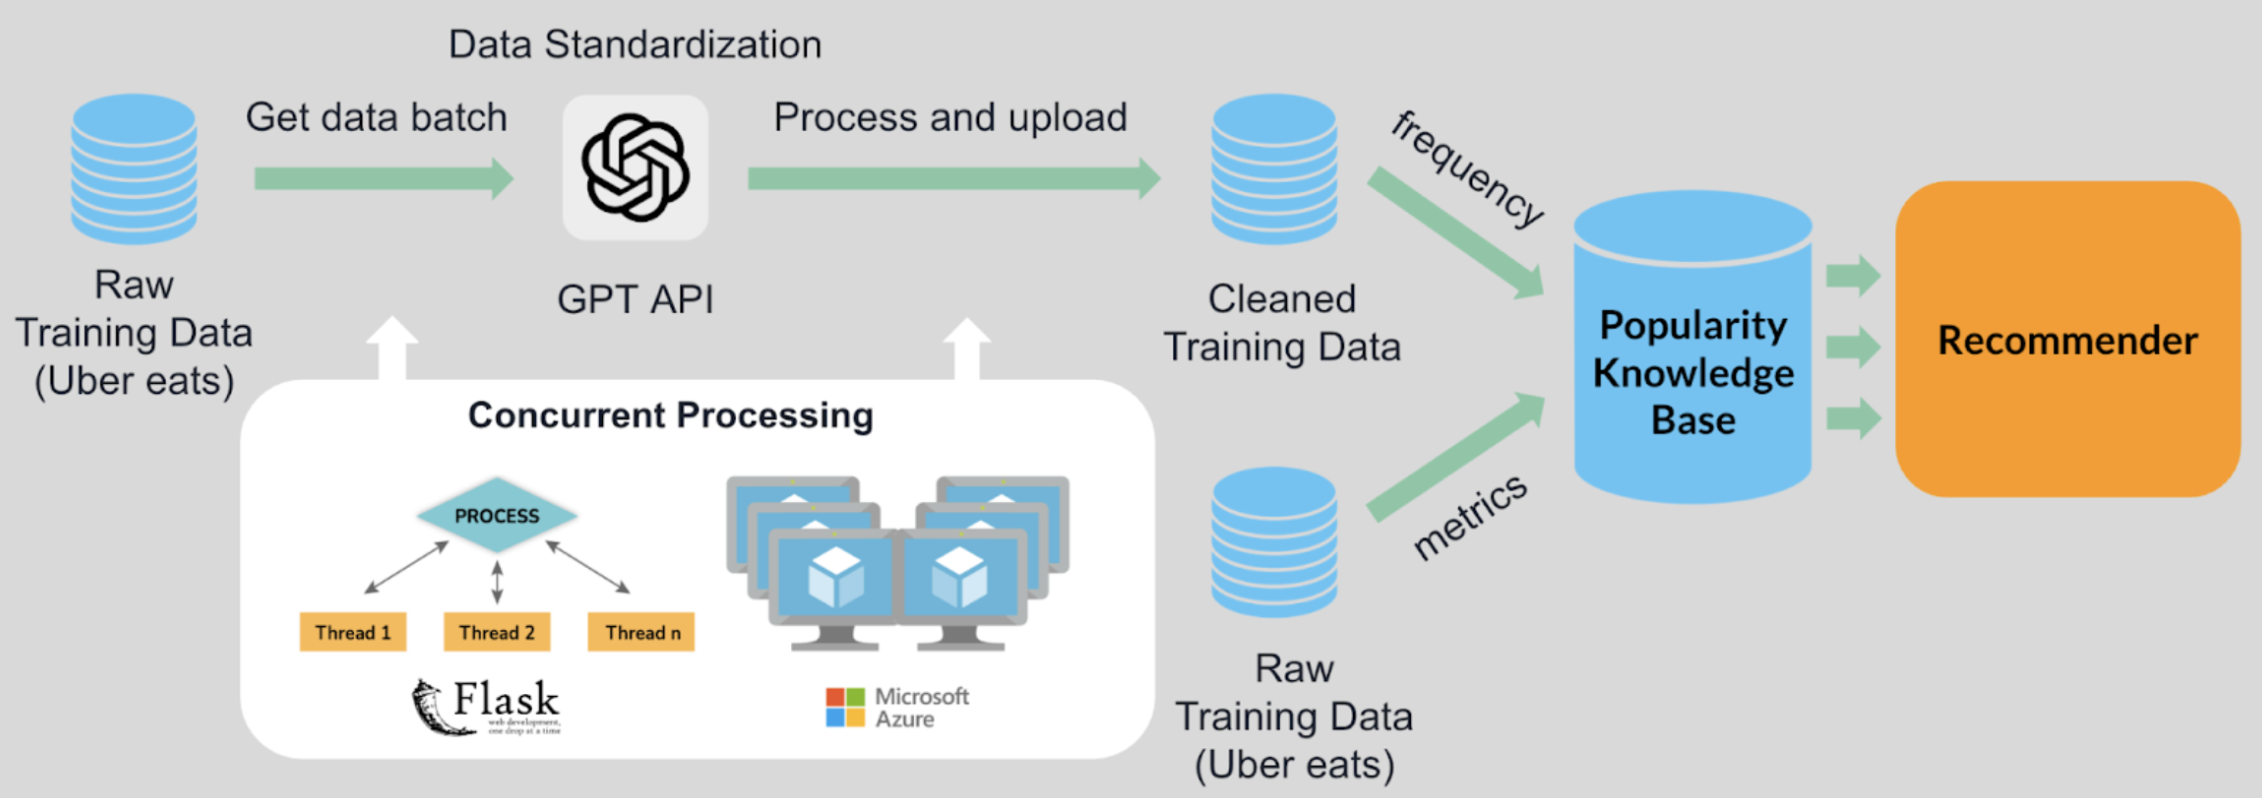
\includegraphics[width=0.8\textwidth,height=\textheight]{../image/final_3_training_pipline.png}

}

\end{figure}%

\begin{enumerate}
\def\labelenumi{\arabic{enumi}.}
\tightlist
\item
  Data Cleaning: Due to inconsistencies in the raw menu data from Uber
  Eats, we implemented preprocessing procedures. Since dishes were named
  differently across restaurants, we developed a semantic
  standardization pipeline powered by the GPT API to normalize dish
  names and group similar items under unified labels.
\item
  Cleaning Deployment: This standardization process was deployed using a
  Flask-based batch-processing mechanism to enable concurrent
  processing. The Heymate engineering team will explore Azure as a
  potential option for faster and automated deployment. Each batch of
  raw data was processed and uploaded to generate a cleaned dataset.
\item
  Scoring and Knowledge Base: Once the data was standardized, we joined
  each menu item with key popularity metrics. This aggregated table will
  be stored and used to calculate popularity scores, which will be
  discussed in detail in a later section.
\end{enumerate}

For the model testing dataset (Figure~\ref{fig-testing-pipline}), the
similar logic is applied here as Heymate's internal database also
exbihits some extent of quality issues (shown in
Figure~\ref{fig-null-internal}). The standardized input will pass
through the recommender system to generate top-rated dish
recommendations.

\begin{figure}

\caption{\label{fig-null-internal}Null Entries in internal dataset
(Model Testing Data)}

\centering{

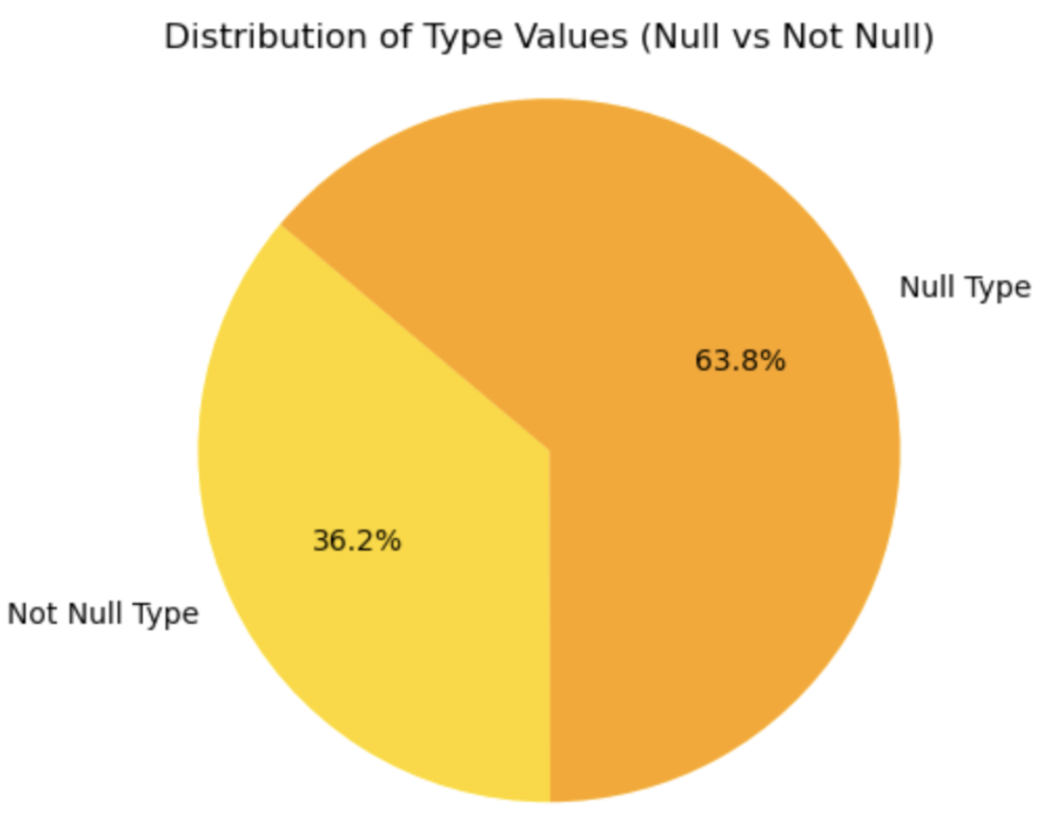
\includegraphics[width=0.6\textwidth,height=\textheight]{../image/final_2_null_internal.png}

}

\end{figure}%

\begin{figure}

\caption{\label{fig-testing-pipline}Solution Pipeline (Model Testing)}

\centering{

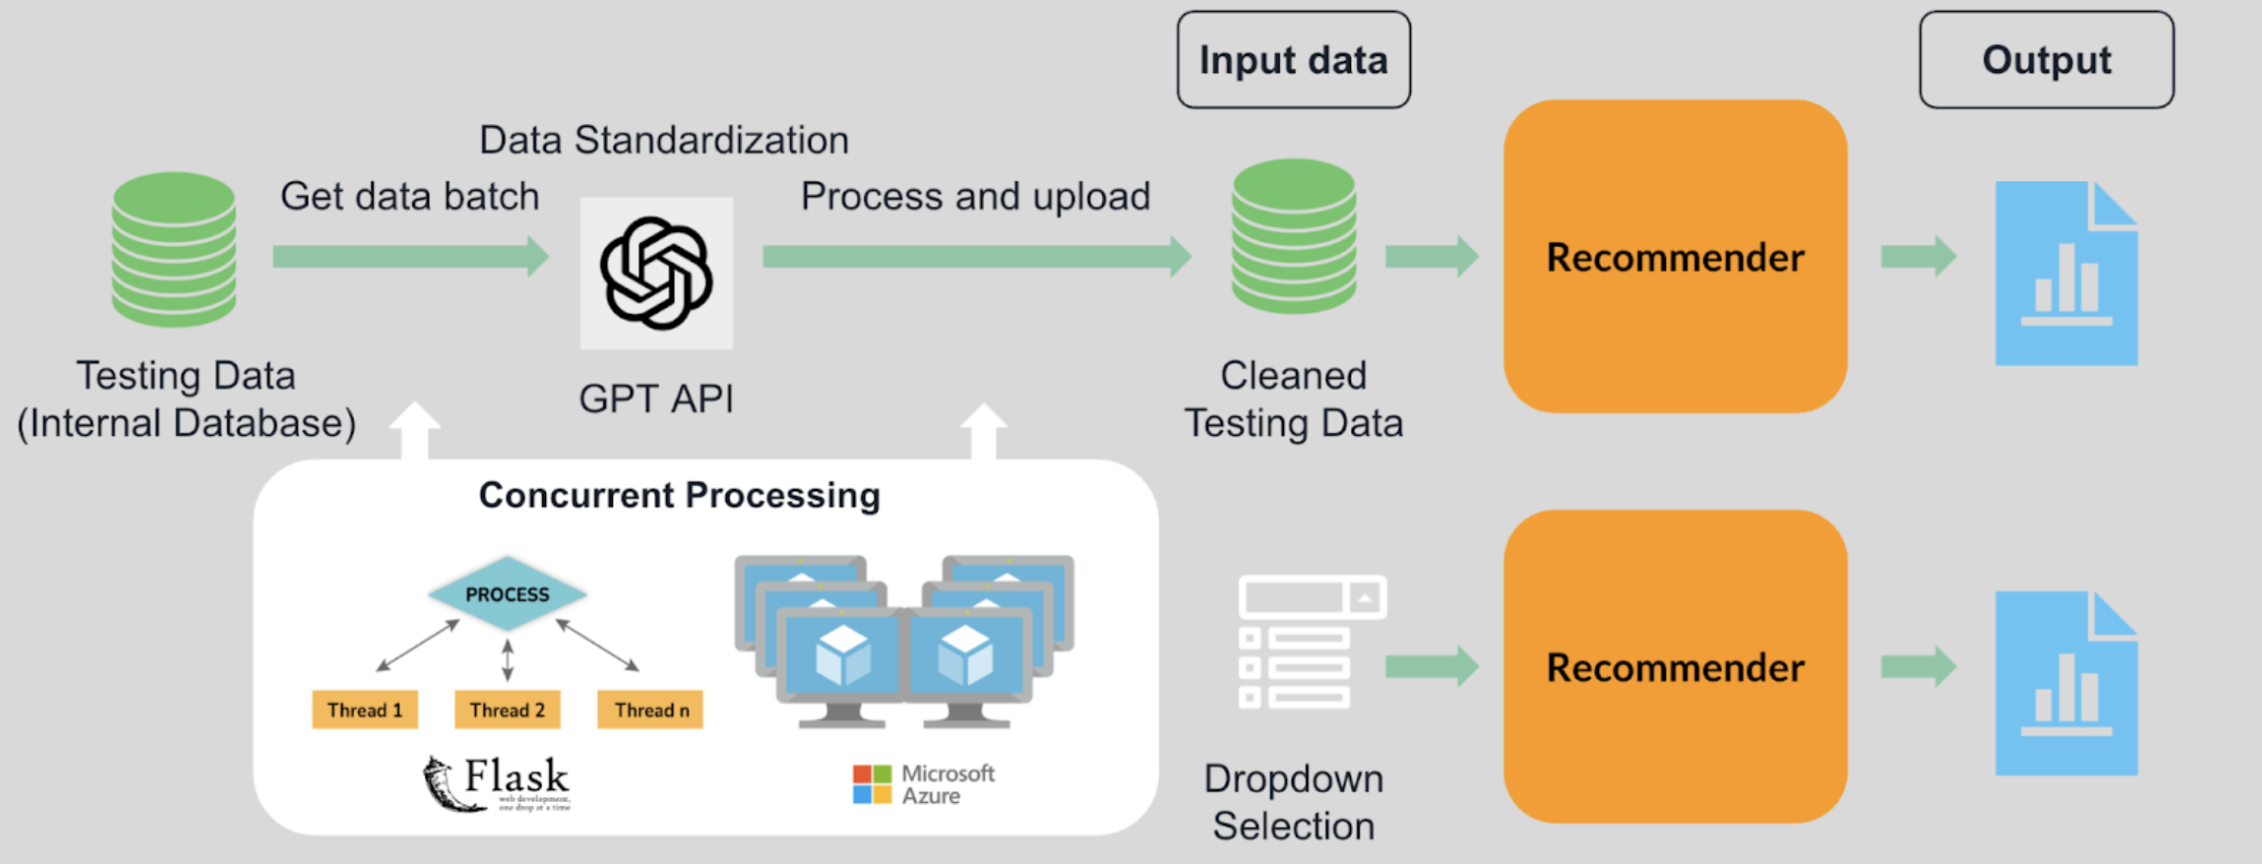
\includegraphics[width=0.8\textwidth,height=\textheight]{../image/final_4_testing_pipline.png}

}

\end{figure}%

\subsection{Data Cleaning Module}\label{data-cleaning-module}

After reviewing the overall pipeline, we now take a closer look at the
data cleaning component, which plays a key role in addressing
inconsistencies in menu dish names and enhancing the quality of
downstream recommendations. Specifically, we want to address following
issues:

\begin{itemize}
\tightlist
\item
  Mixed languages: Many item names contain both English and non-English
  text (Figure~\ref{fig-cleaning-challenge}).
\item
  Inconsistent restaurant types: Broad categories (e.g.~``American'')
  are mixed with specific terms (e.g.~``wings'', ``sandwich''), making
  aggregation difficult.
\item
  Combo indicators: Expressions such as ``Combo'', ``Set of Two'', or
  ``Family Meal'' are used inconsistently, complicating identification.
\item
  Quantity terms: Words like ``6 Pc'' add additional noise and make
  parsing less accurate.
\end{itemize}

\begin{figure}

\caption{\label{fig-cleaning-challenge}Cleaning Challenge Example}

\centering{

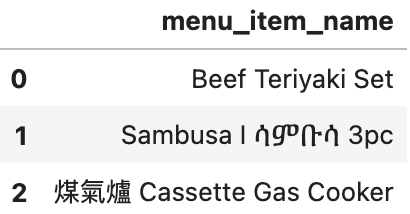
\includegraphics[width=0.3\textwidth,height=\textheight]{../image/final_9_cleaning_challenge.png}

}

\end{figure}%

Without resolving these issues, it would have been impossible to run any
structured analysis across restaurants at scale. Since our project
timeline are relatively tight, we decided to utilize GPT API as it can
achieve semantic inference, format alignment, as well as language
processing in a more efficient manner while maintaining relativeky great
quality. Therefore, we developed a prompt-engineering pipeline that
includes two main parts:

\begin{enumerate}
\def\labelenumi{\arabic{enumi}.}
\tightlist
\item
  System prompt: Defines the input and output schema as well as cleaning
  rules, such as how to identify the core dish name, extract up to five
  descriptors, determine whether an item is a combo, and standardize the
  restaurant type.
\item
  User prompt: Feeds batches of raw menu rows into the model in a list
  of dictionary format.
\end{enumerate}

The GPT model returns structured output for each menu item, including
(Figure~\ref{fig-cleaned-example}):

\begin{itemize}
\tightlist
\item
  \texttt{dish\_base}: core identity (e.g.~``fried rice'').
\item
  \texttt{dish\_flavor}: tags like cooking method or toppings
  (e.g.~{[}``chicken''{]}).
\item
  \texttt{is\_combo}: boolean indicating if the item is a combo.
\item
  \texttt{restaurant\_type\_std}: standardized restaurant type aligned
  with Google Maps Food and Drinks category.
\end{itemize}

\begin{figure}

\caption{\label{fig-cleaned-example}Cleaned Menu Iten Example}

\centering{

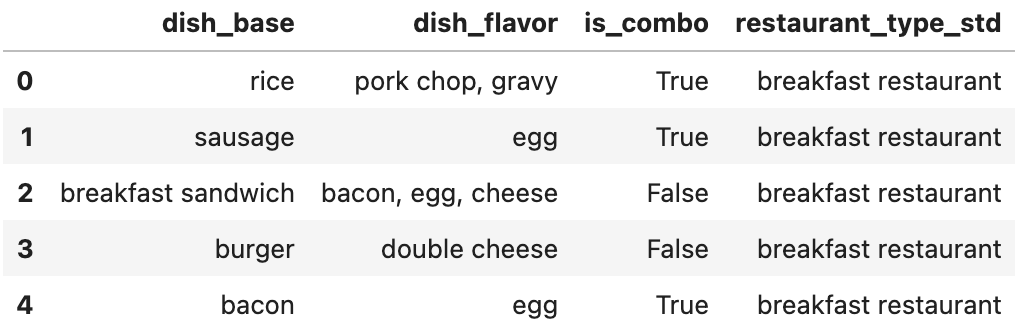
\includegraphics[width=0.7\textwidth,height=\textheight]{../image/final_10_cleaned_example.png}

}

\end{figure}%

To ensure extraction quality and reliability, we iteratively refined our
prompt engineering strategy:

\begin{itemize}
\tightlist
\item
  Required vs.~optional fields: We clearly specified which fields
  (e.g.~item name) must be present, and which are optional (e.g.~menu
  description). When optional fields were missing, the model was
  instructed to infer based on other inputs.
\item
  Formatting rules: We enforced strict formatting in the output,
  including lowercase, singular, American English spellings, to ensure
  consistency.
\item
  Controlled restaurant type output: We constrained the model to select
  from a fixed list of restaurant types aligned with Google Maps Food
  and Drinks categories.
\item
  Combo identification: We embedded recognition logic for different
  combo indicators, such as ``set of'', ``combo'', or ``family meal''.
\item
  Prompt length optimization: Through iterative testing, we shortened
  prompt size while maintaining output quality, helping reduce API
  costs.
\item
  Row indexing: Each row in the batch was assigned a unique index to
  link the model's structured output back to other features like rating
  or score.
\end{itemize}

With this module, we were able to clean inconsistent menu data into a
structured format suitable for downstream analysis and recommendation.

\subsection{Recommendations Algorithm}\label{recommendations-algorithm}

\begin{figure}

\caption{\label{fig-rec-flow}Recommendations Workflow}

\centering{

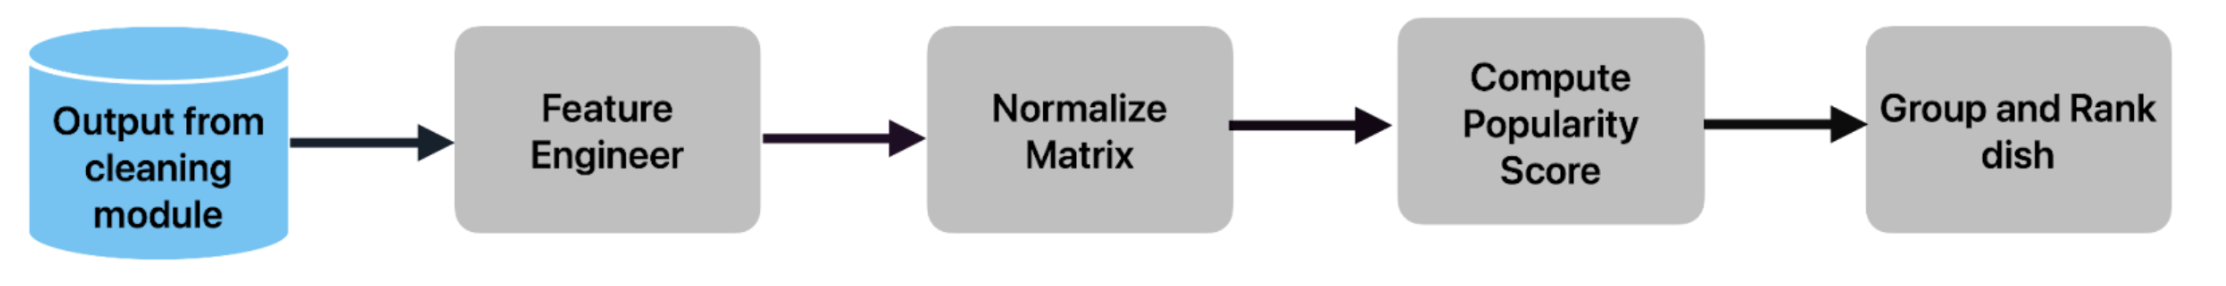
\includegraphics[width=0.8\textwidth,height=\textheight]{../image/final_5_recommendation_flow.png}

}

\end{figure}%

\subsubsection{Feature Integration}\label{feature-integration}

Once the LLM produces cleaned menu data (in table
\texttt{cleaned\_menu\_mds}), we proceeded to feature integration,
enriching this data with relevant popularity metrics. At this stage, we:

\begin{itemize}
\tightlist
\item
  Joined the cleaned Uber Eats menu data (text data) with popularity
  metrics in the original Uber Eats metadata table
  \texttt{Restaurants\_mds}, which contains rating counts and rating
  scores.
\item
  This step allowed us to bring back three key popularity indicators
  that were temporarily removed during cleaning:

  \begin{itemize}
  \tightlist
  \item
    Number of Ratings: how many users rated the dish
  \item
    Average Rating: the restaurant average rating score given by users
  \item
    Item Frequency: how often a dish appears, counting occurrences
    grouped by dish base, dish flavor, and restaurant type
  \end{itemize}
\item
  We also removed entries where \texttt{is\_combo\ ==\ True} to avoid
  noise in popularity estimates.
\end{itemize}

The resulting dataset forms the \textbf{core knowledge base}, a
structured, popularity-aware version of Uber Eats data, on which all
recommendations are based.

\subsection{Normalize Matrix}\label{normalize-matrix}

For popularity score calculation, as the raw values of frequency or
rating counts can be heavily skewed or on different scales. We applied
\textbf{MinMaxScaler} to rescale them to the {[}0, 1{]} range to ensure
that the three indicators (rating counts, rating scores, frequency) are
comparable and balanced.

Normalized columns include:

\begin{itemize}
\tightlist
\item
  \texttt{freq\_scaled}: normalized frequency of the dish
\item
  \texttt{rating\_scaled}: normalized count of user ratings
\item
  \texttt{score\_scaled}: normalized average user rating
\end{itemize}

This step creates a uniform basis for computing the final popularity
score.

\subsection{Compute Popularity Score}\label{compute-popularity-score}

We calculate a weighted popularity score for each dish as follows:

\texttt{popularity\_score\ =\ (0.2\ *\ freq\_scaled\ +\ 0.6\ *\ rating\_scaled\ +\ 0.2\ *\ score\_scale)}

These weights were selected based on exploratory testing and domain
intuition from the partner, prioritizing the number of reviews as a
strong signal of customer engagement, an approach supported by industry
practices/research in similar recommendation systems (Chitalia (2023)
Al-Rubaye and Sukthankar (2020))

\begin{itemize}
\tightlist
\item
  \textbf{60\% rating count: (\texttt{rating\_scaled})} Measures how
  many people have reviewed; we viewed it as the strongest proxy of
  broad customer engagement.
\item
  \textbf{20\% average score: (\texttt{score\_scaled})} captures
  perceived quality but is often biased by low volume.
\item
  \textbf{20\% frequency: (\texttt{freq\_scaled})} reflects widespread
  presence on menus but doesn't always indicate desirability.\\
  All computed scores are stored in a SQL table:
  \texttt{cleaned\_menu\_with\_popularity} This becomes the knowledge
  base table used for filtering and recommendations.
\end{itemize}

\subsection{Group and Rank Dishes (Filtering \& Output
Logic)}\label{group-and-rank-dishes-filtering-output-logic}

At recommendation time, the system:

\begin{enumerate}
\def\labelenumi{\arabic{enumi}.}
\tightlist
\item
  Accepts input from a restaurant partner (up to 3 restaurant types)
\item
  Filters the knowledge base (\texttt{cleaned\_menu\_with\_popularity})
  using:

  \begin{itemize}
  \tightlist
  \item
    Exact matches on restaurant\_type\_std
  \item
    Filters out duplicate dishes (e.g.~same base/flavor combo for the
    same type)
  \end{itemize}
\item
  For multi-type requests, the popularity scores are averaged across the
  selected types
\item
  Dishes are then ranked based on their average popularity score
\end{enumerate}

Finally, the top N dishes (configurable) are returned as output.

\subsubsection{Clarification on Filtering
Scope}\label{clarification-on-filtering-scope}

Currently, our system supports \textbf{structured filtering only}
specifically, by one to three restaurant\_type\_std values (e.g.~``pizza
restaurant''). These types are extracted during LLM cleaning and matched
exactly during the filtering process. This was inspired by best
practices in popularity-based recommenders, which focus on transparency
and operational simplicity in early-stage deployment Sreekala (2020). At
this stage, we do \textbf{not} support:

\begin{itemize}
\tightlist
\item
  Keyword-based filtering (e.g.~searching for ``pepperoni'')
\item
  Semantic/embedding-based matching (e.g.~interpreting ``comfort food''
  or ``something spicy'')
\item
  GPT-powered fuzzy search at recommendation time
\end{itemize}

This was a deliberate choice to prioritize \textbf{transparency,
control,} and \textbf{execution speed} in our MVP. Additionally, our
dataset, though enriched and cleaned, lacked consistent free-text
queries or labelled user intent, which made implementing semantic search
or GPT-based query interpretation less feasible at this stage.

\section{Example Use Case: Recommending for a Pizza
Restaurant}\label{example-use-case-recommending-for-a-pizza-restaurant}

To demonstrate how the recommendation engine works in practice, we
include a use case where a partner restaurant is identified as a
\textbf{``pizza restaurant''}. The system filters all dishes from our
cleaned Uber Eats knowledge base that match this restaurant type and
scores each based on its normalized rating score, frequency, and rating
count. The weighted score is then used to rank the items, returning the
top 10 most relevant dishes.

As shown in the figure below Figure~\ref{fig-rec-example}, the
top-ranked items for a pizza restaurant include popular classics such
as:

\begin{itemize}
\tightlist
\item
  Pizza (cheese) and Pizza (pepperoni) --- widely rated and highly
  frequent across menus.
\item
  Pizza (meat lover) and Spaghetti (meatball) --- dishes with consistent
  performance.
\item
  Less expected but still relevant items like Papadia (parmesan crust)
  also appear due to strong metric combinations.
\end{itemize}

\begin{figure}

\caption{\label{fig-rec-example}Recommendations For a Pizza
Restaurant''}

\centering{

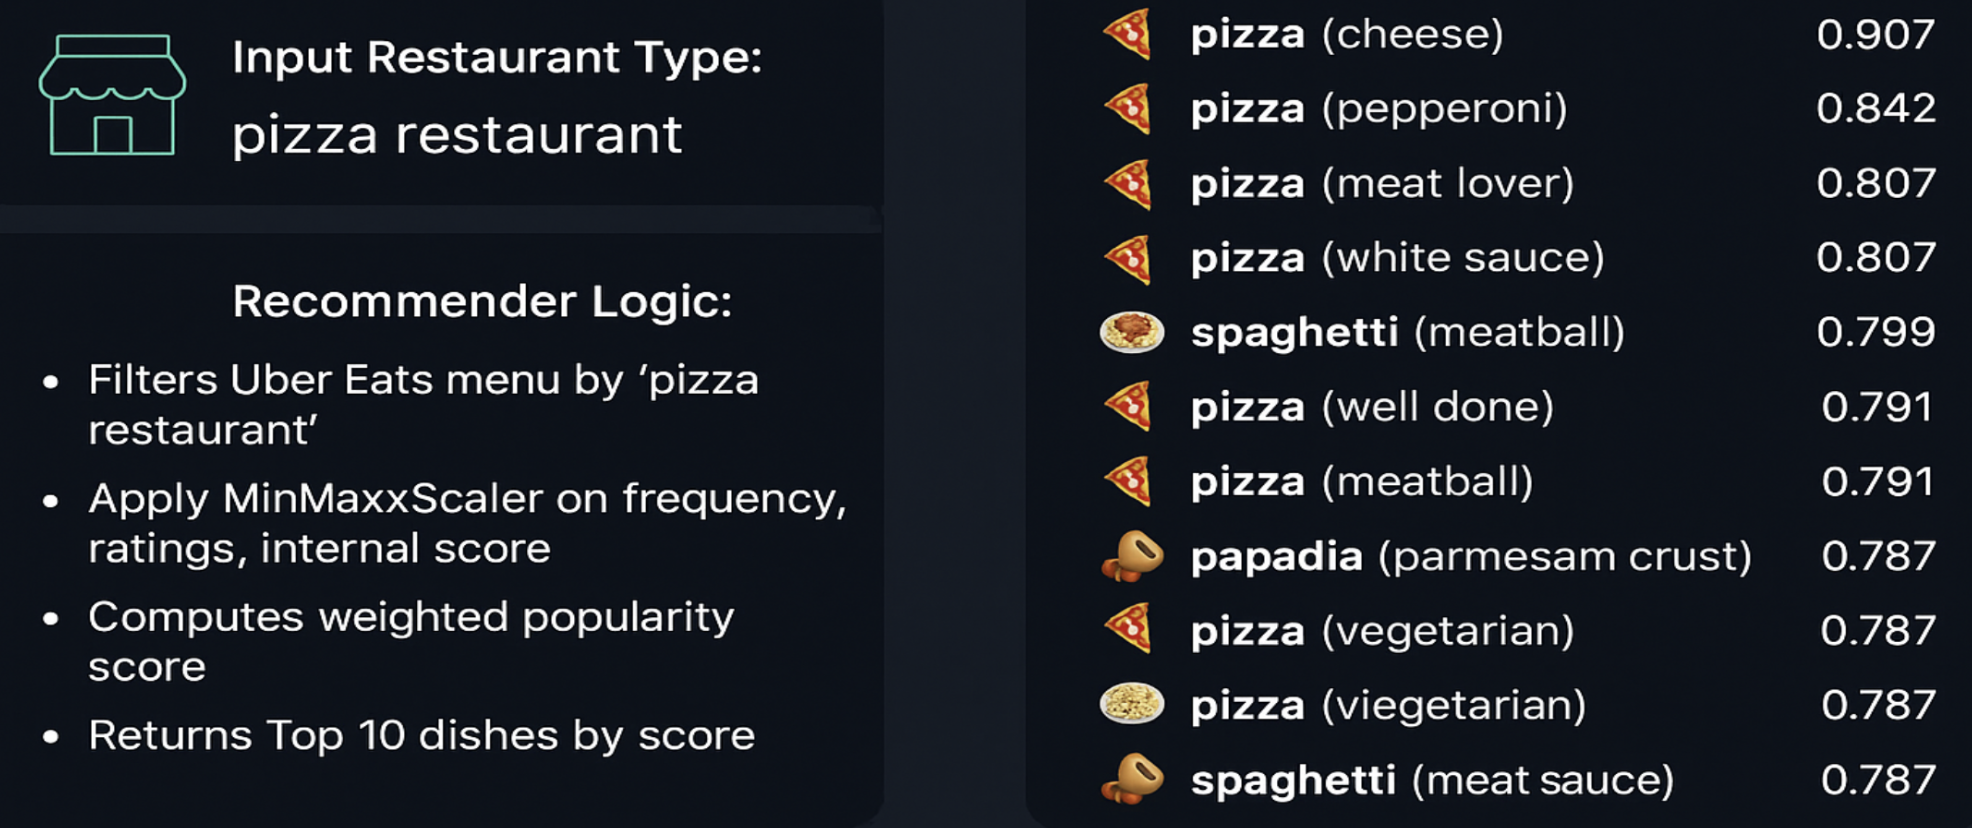
\includegraphics[width=0.8\textwidth,height=\textheight]{../image/final-7-rec-example.png}

}

\end{figure}%

\subsection{Visualization Demo: Surfacing Actionable
Recommendations}\label{visualization-demo-surfacing-actionable-recommendations}

\begin{figure}

\caption{\label{fig-viz-demo}Visualization Demo''}

\centering{

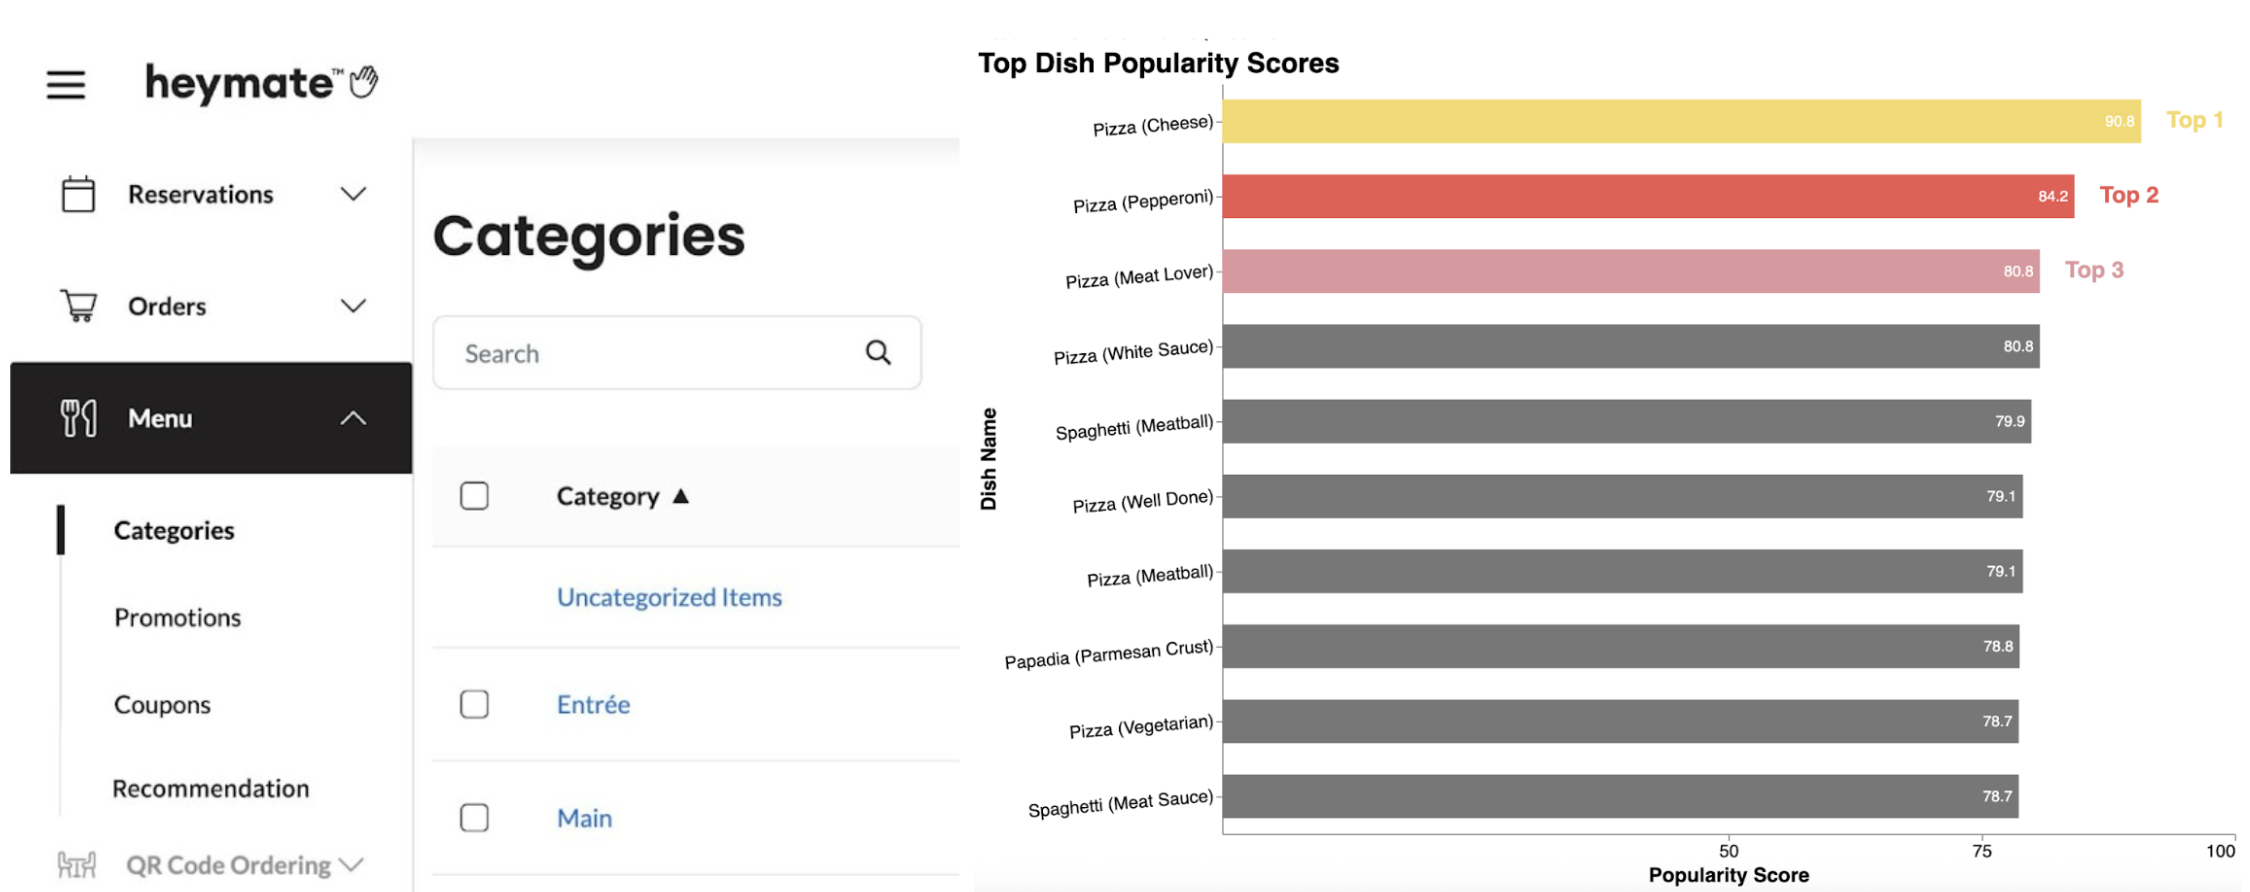
\includegraphics[width=0.8\textwidth,height=\textheight]{../image/final-8-viz.png}

}

\end{figure}%

To make our recommendation results interpretable and actionable, we
built a two-part visualization:

\subsubsection{CRM System Integration
Mockup}\label{crm-system-integration-mockup}

On the left of Figure~\ref{fig-viz-demo}, we show a conceptual UI for
how this recommendation module could be embedded in the Heymate CRM by
the Heymate engineering team. This allows restaurant managers to easily
access insights from their dashboard, specifically under the
``Recommendation'' tab, alongside other operational menus.

\subsubsection{Recommendation Output
Visualization}\label{recommendation-output-visualization}

On the right of Figure~\ref{fig-viz-demo} is an Altair-based bar chart
showcasing the top dishes sorted by computed popularity score. Key
design features include:

\begin{itemize}
\tightlist
\item
  Top 3 highlights using Heymate brand colours (yellow, red, rose).
\item
  Pop score bars are annotated directly with percentage labels.
\item
  Hover tooltips for dish name and score for ease of exploration.
\item
  Combined label (dish base + flavor) for intuitive comprehension.
\end{itemize}

This visualization not only validates that our scoring pipeline works
but also provides a clear and professional way for stakeholders to
compare and act on dish performance. It is also exportable as a
standalone HTML component and ready for dashboard integration.

\section{How to Use the Data Product}\label{how-to-use-the-data-product}

We designed this data product to support Heymate's internal team and
clients in making data-informed menu decisions.

\subsection{Intended Usage}\label{intended-usage}

Heymate can utilize this tool in two primary ways:

\begin{itemize}
\tightlist
\item
  Internal Use Mode:

  \begin{itemize}
  \tightlist
  \item
    Data Update \& Validation: When a new data source becomes available,
    the internal team can upload and process it through the system to
    evaluate performance with updated inputs.
  \item
    Testing \& Iteration: By inputting internal client restaurant types,
    internal users can assess the quality of dish name cleaning and
    observe how the system generates standardized output. This enables
    iterative refinement and ensures reliability before onboarding new
    clients.
  \end{itemize}
\item
  Client-Facing Deployment: On the frontend, a client can simply select
  their restaurant type (e.g.~``pizza restaurant''), and the system
  returns a list of top recommended dishes based on aggregated
  popularity metrics from similar restaurants. This empowers merchants
  to make data-driven menu decisions aligned with current market trends.
\end{itemize}

Overall speaking, to enable a scalable, end-to-end pipeline that
supports both internal testing and client-facing deployment, we applied
several key data science techniques. Below, we highlight three methods
that were critical to addressing real-world data challenges.

\section{Data Science Methods}\label{data-science-methods}

We applied many data science techniques in our capstone project and are
highlighting 3 here:

\begin{itemize}
\tightlist
\item
  LLM Integration
\item
  Distributed Deployment
\item
  Materialized View
\end{itemize}

\subsection{LLM Integration}\label{llm-integration}

We leveraged large language models (LLMs) to clean and standardize the
menu data. The raw data was not available for direct use in our
recommendation system due to inconsistencies in formatting, spelling
variations, and the presence of multiple languages. By integrating LLMs,
we were able to extract key information of dish bases and dish flavors,
from item names, categories, and descriptions with high accuracy. Even
in the case when the description is missing, the LLMs can still infer
the information from the item name and category, as well as the context
of the restaurant name.

\subsubsection{Limitation}\label{limitation}

This approach requires payment for API usage. After evaluating
trade-offs between computational power and cost, we chose to use the
\textbf{ChatGPT-4o mini} model.

\subsubsection{Alternative Methods
Considered}\label{alternative-methods-considered}

\begin{itemize}
\tightlist
\item
  Regular Expressions: Effective for extracting structured patterns, but
  not feasible here due to inconsistent formatting and multilingual
  input.
\item
  Custom Deep Learning Model: While potentially powerful, this would
  require labelled training data and significant time and computational
  resources. We don't have such resources within our project scope.
\item
  Locally Deployed LLM: This could reduce long-term costs, but setup and
  maintenance would bring practical challenges within our capstone
  timeline.
\end{itemize}

\subsection{Distributed Deployment}\label{distributed-deployment}

Our project involved processing a large dataset, over 3 million rows
from the Uber Eats dataset. Cleaning this data sequentially would have
taken approximately 5,000 hours, which was not feasible within our
timeline. To solve this, we implemented a distributed deployment
infrastructure to significantly speed up processing. We designed and
deployed an HTTP-triggered function to process data in batches. Each
instance is triggered via a web request, with the batch range passed as
parameters. The system logs the task status at both the start and end of
execution. To monitor tasks internally, we also built a dashboard in
Looker Studio. Initially, we planned to deploy using Azure Functions on
our partner's cloud infrastructure. However, due to security
configuration challenges, we were unable to proceed with this plan. As a
fallback, we deployed the system locally using the Flask framework and
ran up to 20 worker instances concurrently, achieving a 20x speedup.

\subsubsection{Limitation}\label{limitation-1}

The number of concurrent worker instances is limited by the ChatGPT API
rate limit.

\subsubsection{Alternative Approaches
Considered}\label{alternative-approaches-considered}

We evaluated other cloud deployment solutions, such as EC2 from Amazon
Web Services and Google Cloud Functions from the Google Cloud Platform.
However, our partner uses Microsoft Azure, and we prioritized
consistency within that ecosystem. In the future, our partner's
engineering team plans to migrate our local deployment to Azure
Functions, once security configurations are in place.

\subsection{Materialized View}\label{materialized-view}

A Materialized View (also known as a Persistent Derived Table) is a
database optimization technique that stores the result of a query as a
physical table. This allows for much faster data retrieval by avoiding
repeated computation over large datasets. Initially, it took around 6
minutes to generate a restaurant recommendation due to the volume of
data. Such delays are unacceptable in production, especially since the
recommendation module will eventually be integrated into the partner's
CRM system. To optimize query performance, we implemented a materialized
view to cache pre-computed results. This optimization reduced runtime
from 6 minutes to just 3 seconds.

\subsubsection{Limitations}\label{limitations}

\begin{itemize}
\tightlist
\item
  Additional Storage Cost: The materialized view aggregates data from
  the original 3-million-row table, incurring some storage cost.
  However, this is minimal relative to the base data and is not a major
  concern.
\item
  Maintenance and Updates: When new data is ingested into the model
  input pipeline, the materialized view must be refreshed. To handle
  this, we established an automated workflow that updates the
  materialized view upon the successful completion of each data
  ingestion task.
\end{itemize}

\section{Justification Over Other
Products/Interfaces}\label{justification-over-other-productsinterfaces}

There are existing solutions that rely entirely on LLMs to build AI
agents for restaurant recommendations. In these systems, user inputs are
translated into prompts and sent to an LLM, which generates
recommendations based on its internal knowledge.

However, this approach has several clear limitations:

\begin{enumerate}
\def\labelenumi{\arabic{enumi}.}
\tightlist
\item
  LLMs are transformer-based models and are not well-suited for handling
  structured logic or computations involving large-scale tabular data.
\item
  Interpretability is low: these systems often function as black boxes,
  making it difficult to understand or explain how the recommendations
  are generated.
\item
  Lack of real market data: These models typically do not incorporate
  up-to-date or domain-specific datasets. In contrast, our system is
  built on a dataset of over 3 million real menu records, providing a
  much more grounded and data-driven foundation for recommendations.
\end{enumerate}

\section{Conclusions and
Recommendations}\label{conclusions-and-recommendations}

\subsection{What Problem Were We
Solving?}\label{what-problem-were-we-solving}

Heymate seeks to empower its restaurant partners by offering data-driven
menu recommendations that encourage customer return visits. However,
partners often lack clear insights into which menu items perform well
across the market and why. Our project aimed to close this gap by
designing a popularity-based recommendation system that scores dishes
based on the number of ratings, average rating scores, and frequency
across menus, offering partners a transparent foundation for data-backed
decision-making.

\subsection{How Does Our Solution Address
It?}\label{how-does-our-solution-address-it}

We developed a full-stack pipeline that:

\begin{itemize}
\tightlist
\item
  Cleans and standardizes restaurant menu data using LLMs,
\item
  Joins the cleaned internal menu with Uber Eats data to enrich it with
  restaurant-level popularity signals,
\item
  Computes a weighted popularity score using MinMaxScaler across three
  metrics,
\item
  Filters and ranks menu items based on restaurant type(s),
\item
  Visualizes the results in an interactive Altair chart for use in
  Heymate's CRM.
\end{itemize}

This product functions well as a minimum viable recommendation engine,
particularly for restaurant partners without access to historical
purchase data. Its transparent logic and simple interface make it
accessible for immediate use and experimentation.

\subsection{Limitations}\label{limitations-1}

While our data product offers a practical solution for transforming raw
menu data into structured insights, several limitations remain:

\begin{itemize}
\tightlist
\item
  \textbf{Popularity Bias:} Our current popularity scoring system relies
  on static metrics due to the lack of real transaction data. This makes
  it a proxy measure and may not fully reflect true customer
  preferences. The score could be further improved by incorporating
  additional quantitative features like price, review volume, or order
  frequency if available in the future.
\item
  \textbf{Static Reference:} Our analysis is currently based on static
  snapshots of menu data. Without timestamped records, we are unable to
  capture how item popularity or menu composition evolves. This limits
  our ability to detect trends such as seasonal specials or emerging
  bestsellers.
\item
  \textbf{Hard Filtering:} Restaurant type filtering is an exact match
  only (e.g.~``pizza restaurant''), limiting support for broader or
  fuzzy queries like ``comfort food'' or ``date night meals''. A more
  flexible filtering mechanism could improve the versatility of the
  tool.
\item
  \textbf{Evaluation Challenge:} Due to limited deployment and lack of
  real-time feedback from users, our validation process is based on
  illustrative case studies (e.g.~the pizza restaurant example). While
  useful for demonstration, A/B testing or real user feedback would be
  necessary to confirm the real-world effectiveness of the tool.
\item
  \textbf{Scalability Constraint:} Although our local pipeline performs
  well, we haven't deployed it to Azure yet due to resource and security
  constraints. As a result, the system is not yet scalable enough for
  real-time or production use cases.
\item
  \textbf{Lack of Granular Personalization:} While our system
  standardizes restaurant types (e.g.~``Chinese restaurant''), it does
  not yet support finer-grained classification at the sub-type level
  (e.g.~``Szechuan,'' ``Cantonese''). Additionally, the recommender
  ignores important factors such as local popularity, pricing, and
  user-specific preferences. These limitations reduce the system's
  ability to deliver tailored insights for diverse audiences.
\end{itemize}

\subsection{Recommendations for
Heymate}\label{recommendations-for-heymate}

To evolve this prototype into a production-ready recommender, we
recommend:

\begin{enumerate}
\def\labelenumi{\arabic{enumi}.}
\tightlist
\item
  Temporal Tracking: Incorporate timestamped data to uncover seasonal
  patterns and trends.
\item
  Restaurant Feedback Loop: Integrate feedback from partner restaurants
  to refine recommendations over time.
\item
  Semantic Filtering: Support flexible, natural-language queries using
  embeddings or GPT-powered matching.
\item
  Cloud Deployment: Deploy to Azure to support scalability and integrate
  directly with Heymate's CRM system.
\item
  Subtype Extraction: Enhance LLM outputs with more detailed tags
  (e.g.~``spicy,'' ``gluten-free,'' ``vegan'') for deeper filtering.
\item
  Evaluation Framework: Design structured evaluations using click data,
  client interviews, or business KPIs to measure impact.
\end{enumerate}

Our product lays a solid foundation for \textbf{scalable, transparent},
and \textbf{explainable menu recommendations}. With further iteration,
it can evolve into a dynamic and adaptive system that supports Heymate's
long-term vision for partner success.

\newpage{}

\section*{References}\label{references}
\addcontentsline{toc}{section}{References}

\phantomsection\label{refs}
\begin{CSLReferences}{1}{0}
\bibitem[\citeproctext]{ref-alrubaye2020github}
Al-Rubaye, S., and G. Sukthankar. 2020. {``Popularity-Based Ranking of
GitHub Repositories.''} \emph{IEEE}.
\url{https://ieeexplore.ieee.org/document/9458206}.

\bibitem[\citeproctext]{ref-chitalia2023yelp}
Chitalia, A. 2023. {``Yelp Popularity Score Calculator.''}
\url{https://scholarworks.sjsu.edu/etd_projects/1261}.

\bibitem[\citeproctext]{ref-sakib2023ubereats}
Sakib, Ahmed Shahriar. 2023. {``Uber Eats USA Restaurants and Menus.''}
\url{https://www.kaggle.com/datasets/ahmedshahriarsakib/uber-eats-usa-restaurants-menus}.

\bibitem[\citeproctext]{ref-keshetti2020popularity}
Sreekala, Keshetti. 2020. {``Popularity-Based Recommendation System.''}
\url{https://www.researchgate.net/publication/355773477}.

\end{CSLReferences}




\end{document}
